
%sudo apt-get install texlive-bibtex-extra
%Word counts: pdftotext WBVFM_IntroPar.pdf - | wc -w
\documentclass{article}\usepackage[]{graphicx}\usepackage[]{color}
%% maxwidth is the original width if it is less than linewidth
%% otherwise use linewidth (to make sure the graphics do not exceed the margin)
\makeatletter
\def\maxwidth{ %
  \ifdim\Gin@nat@width>\linewidth
    \linewidth
  \else
    \Gin@nat@width
  \fi
}
\makeatother

\usepackage{Sweave}


\usepackage{float}
\usepackage{wrapfig}
\usepackage{hyperref}
\usepackage{authblk}
\usepackage{tablefootnote}
\usepackage{graphicx}
\usepackage[backend=bibtex, style=nature, citestyle=authoryear]{biblatex}
\bibliography{WBVFM_IntroPar}
\newenvironment{knitrout}{}{}  %just a dummy environment


\makeatletter
\newcommand\gobblepars{%
    \@ifnextchar\par%
        {\expandafter\gobblepars\@gobble}%
        {}}
\makeatother



\author[1]{Daniel Runfola\thanks{dsmillerrunfol@wm.edu}}
\author[1]{Ariel BenYishay\thanks{abenyishay@wm.edu}}
\author[2]{Jeff Tanner\thanks{jtanner@worldbank.org}}
\author[3]{Graeme Buchanan\thanks{graeme.buchanan@rspb.org.uk}}
\author[4]{Jyothy Nagol\thanks{jnagol@umd.edu}}
\author[5]{Matthias Leu\thanks{mleu@wm.edu}}
\author[1]{Seth Goodman \thanks{smgoodman@wm.edu}}
\author[1]{Rachel Trichler\thanks{rbtrichler@wm.edu}}
\author[1]{Rob Marty\thanks{ramarty@email.wm.edu}}

\affil[1]{Institute for the Theory and Practice of International Relations, The College of William and Mary}
\affil[2]{Independent Evaluation Group, World Bank}
\affil[3]{Center for Conservation Science, Royal Society of Birds}
\affil[4]{Global Land Cover Facility, University of Maryland}
\affil[5]{Department of Biology, The College of William and Mary}

\renewcommand\Authands{ and }

\title{A top-down approach to estimating spatially heterogeneous impacts of development aid on vegetative carbon sequestration}
\date{\vspace{-5ex}}
\IfFileExists{upquote.sty}{\usepackage{upquote}}{}
\begin{document}
\begin{knitrout}



\maketitle 
\begin{flushleft}
\textbf{Short Title}: Estimating impacts of aid on carbon sequestration\\
\textbf{Keywords}: International Aid, Carbon Sequestration, Causal Identification, Heterogeneous Effects\\
\textbf{Words in Abstract:} 143\\
\textbf{Words in Manuscript:} 2,580\\
\textbf{Number of References:} 14\\
\textbf{Number of Figures and Tables:} 4\\
\textbf{Corresponding Author}:\\
Dr. Daniel Runfola\\
Institute for the Theory and Practice of International Relations, \emph{AidData}
Email: dsmillerrunfol@wm.edu
Telephone: 508.316.9109
Fax: 757.221.4650
\end{flushleft}

\newpage
\section{Abstract}

Since 1945, over \$4.9 trillion dollars of international aid has been allocated (\cite{tierney_more_2011}).
To date there have been no estimates of the regional impact of this aid on the carbon cycle.  
We apply a geographically explicit matching method (\cite{andam_measuring_2008}) to estimate the relative impact of large scale World Bank projects implemented between 2000 and 2010 on sequestered carbon, using a novel and publicly available data set of 41307 World Bank project locations. 
Considering only carbon sequestered due to fluctuations in vegetative biomass caused by World Bank projects, we illustrate the relative impact of World Bank projects on carbon sequestration across  development sectors.
We use this information to illustrate the geographic variation in apparent effectiveness of environmental safeguards (\cite{laurance_reducing_2015}) implemented by the World Bank.
We argue that sub-national data can help identify geographically heterogeneous impact effects, and highlight the methodologic barriers which still exist.

\newpage
\section{Introduction}

International recognition of the dual challenges of international development and the mitigation of environmental change is resulting in a large redirection of resources towards developing countries. 
The United States alone has pledged nearly \$4 billion dollars of aid to mitigate climate vulnerability over the next 4 years, and the Paris convention urged donors to target \$100 billion annually by the year 2020 (\cite{royal_united_2015}). 
Coupled with increasing pressure from recipient nations, donors have and continue to introduce more stringent environmental safeguards, including requirements for compliance with national and international regulations, environmental management plans, reforestation goals, and others (\cite{nielson_delegation_2003}, \cite{gutner_explaining_2005}).

\begin{wrapfigure}[17]{r}{0.65\textwidth}\centering
\begin{Schunk}

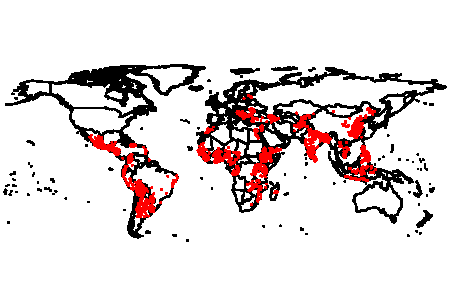
\includegraphics[width=\maxwidth]{figure/WLocs-1} \end{Schunk}
\caption{World Bank IDA and IBRD Project Locations.}
\label{WBLocs}
\vspace{25pt}
\end{wrapfigure}  

\par

Despite these shifts in the policies of donor agencies, there is a gap in empirical studies examining the impacts of these policies on environmental outcomes.  
This letter aims to illustrate an approach to overcoming this gap, as well as highlight many of the remaining methodological challenges.
We specifically examine the impact of large scale World Bank projects on vegetation and subsequent changes in carbon sequestration, leveraging a novel and publicly available data set of 41307 World Bank project locations (see Figure \ref{WBLocs})\footnote{http://aiddata.org/level1/geocoded/worldbank} in conjunction with long-term satellite data quantifying vegetative biomass and a number of spatially-referenced control variables (see table \ref{data_source_table}).

\begin{table}

\begin{tabular}[h]{|p{4.5cm}||p{7cm}|}
\hline
\multicolumn{2}{|c|}{\texttt{Data Sources}} \\
\hline
\textbf{Data Name} & \textbf{Source} \\
\hline
World Bank Geolocations & AidData\begin{math}^{1}\end{math} \\
\hline
Gridded Population of the World & Center for International Earth Science Information Network\tablefootnote{http://sedac.ciesin.columbia.edu/data/collection/gpw-v3/sets/browse} \\
\hline
Nighttime Lights & Defense Meteorological Satellite Program\tablefootnote{Stable Lights retrieved from http://ngdc.noaa.gov/eog/dmsp.html}\\
\hline
Precipitation and Temperature & University of Delaware (\cite{willmott_terrestrial_2001})\tablefootnote{Variables derived from these product included the average precipitation (P) and temperature (T) before a project was implemented (from 1992), the linear trend in P and T from 1992 to the project implementation, the average temperature from the date the project was implemented until the end of the temporal record(2012), and the post-project trend through 2012. Absolute measurements of each variable were also retained. } \\
\hline
Urban Travel Time & European Commission Joint Research Centre\tablefootnote{http://forobs.jrc.ec.europa.eu/products/gam/download.php}\\
\hline
Distance to Rivers & World Wildlife Fund \tablefootnote{http://hydrosheds.cr.usgs.gov/index.php}\\
\hline
Vegetation & NASA LTDR\tablefootnote{http://ltdr.nascom.nasa.gov/cgi-bin/ltdr/ltdrPage.cgi} \\
\hline
Carbon Storage & NASA JPL (\cite{saatchi_benchmark_2011})\tablefootnote{http://click.jpl.nasa.gov/Archive/carbon/ftpdata/carbon/datasets/} \\
\hline
Ecofloristic Zone Carbon Fractions & Oak Ridge National Laboratory (\cite{ruesch_new_2008}) \\
\hline
\end{tabular}
\caption{Data sources used in this analysis.}\label{data_source_table}
\end{table}

\par

We find that while the overall impact of large scale World Bank projects on carbon sequestration appears to be positive, considerable temporal and spatial variation exists in these impacts.
Further, we illustrate the advantages and limitations of a geographically explicit approach to estimating the causal effects of development aid projects, and outline a number of topics for further research.
Finally, we introduce an enhanced, publicly available data set of the global, spatially-explicit distribution of World Bank activities encompassing projects initiated between 1995 and 2014.

\newpage
\section{Methods}

Significant progress has been made on methods which integrate spatial data (i.e., satellite information on forest cover) to quantify the causal impact of interventions (i.e., projects aimed at the prevention of deforestation) (\cite{nelson_effectiveness_2011}).  
These methods largely rely on propensity score and other matching-based methods to select ``control'' cases where no or limited intervention occurred, and match these with similar ``treatment'' cases at the sites of interventions (\cite{andam_measuring_2008}). 
We build on these approaches, implementing a geographically explicit two-stage Propensity Score Matching estimation strategy.
This is motivated by the context of this analysis: specifically, we hypothesize that the impact of World Bank projects is geographically heterogeneous - i.e., a project in the Sahara is unlikely to have the same impact as one in the Amazon.
In this section, we detail one approach which enables researchers to measure impacts in a way which flexibly incorporates geographic heterogeneity.


\subsection{Geographically Explicit Impacts}

First, we truncate the data set to cover World Bank projects from 2000 to 2010 due to limitations of our ancillary information, resulting in a total of 41307 World Bank project locations.
Second, the area of influence within which we anticipate each World Bank project could plausibly have an impact on deforestation is calculated by examining the historic spatial distance at which forest cover is spatially correlated. 
To parameterize this distance, we calculate a Moran's I (\cite{getis_analysis_1992}) score at increasing distances, a metric that measures the degree of spatial autocorrelation for a given variable.
We use this metric to estimate the distance at which spatial autocorrelation is no longer predominant for our outcome measure of forest cover, measured in 1999.  
We argue that this is a highly conservative estimate of the possible area of influence a project could have (i.e., we will tend to over-estimate the buffer size), as it represents the totality of historic spillovers up to the year 1999.

\par
For each of 12 distance bins (between 0 and 2,200 kilometers, in increments of approximately 180km), Moran's I is calculated following:

\begin{equation}
I_h = (\frac{N}{\sum_{i}^{N}\sum_{j}^{N}w_{ij}}) * ((\sum_{i}^{N}\sum_{j}^{N}w_{ij} * (X_{i}-\bar{x}) * \frac{X_{j} - \bar{x}}{\sum_{i}^{N}(X_{i}-\bar{x})})^{2})
\label{EQmoran}
\end{equation}

where \textit{h} represents each spatial bin, \textit{N} the number of spatial units, \textit{i} and \textit{j} are indexes for each unit, \textit{X} is the variable of interest, and \begin{math}W_{ij}\end{math} represents the weights matrix.  
In this application, the weights matrix is specified according to the bin (\textit{h}) being analyzed.  

\par
Once calculated, the distance at which Moran's I is equal to or less than .10 is identified, and used to parameterize a buffer around each project. 
The projects are then subdivided into six different project (sector) types - Health, Environment, Education, Industrial, Infrastructure, and Other.  
Within each of these sectors, projects are further subdivided into three equally-sized monetary bins of "low", "medium", and "high" dollars committed to the project.

\par

Finally, for each high dollar value group-sector combination (6 total groups), a geographically explicit propensity score model is fit.  
This is conducted following a three-stage process which is repeated for every large scale World Bank project, resulting in 13769 total models.
In the first stage, a unit of observation is selected and all World Bank projects that fall within the distance estimated according to the Moran's I are selected as the relevant ``subpopulation'' for that point.
All points within the subpopulation are defined as treated or untreated pending their monetary value - units of observation with a high dollar value (in the upper 33\% for a given sector) are assigned as treated (1), while all projects in the medium and low bins (in the lower 66\% for a sector) are assigned an untreated value (0).

\par
In the second stage, all points within the subpopulation are matched according to a propensity score matching routine.  
Variables matched on can be seen in Table 1, and matches are limited to be within the same sector. 
The propensity scores are calculated once globally following a logit model:

\begin{equation}
T_{i} = \beta_{0} + \sum_{k=1}^{k}(\beta_{k}*x_{i,k})
\label{EQpropensity}
\end{equation}

where \textit{T} is the treatment binary, \textit{i} is the unit of analysis, and \begin{math}\beta_{k}\end{math} are the estimated coefficients for each covariate, \begin{math}x_{k}\end{math}.  

The estimates from this equation are applied to each unit of observation within the subpopulation, and the differences between propensity scores across different units of observation are used to represent a univariate measure of similarity.  
For the set of high dollar value project locations within the area of influence, the optimal set of matched untreated units (without replacement) are identified using a nearest-neighbor optimization (\cite{ho_matchit:_2011}). 
This results in a dataset in which each treated unit is matched with the single control unit most similar to it, with units that have no meaningful comparison dropped from the analysis.
\par

In the third stage, a regression relationship is estimated between the outcome measure (the average LTDR NDVI value in the years after project implementation), the treatment binary, and all available covariates:

\begin{equation}
y_i = \beta_{0} + \theta * T + \sum_{k=1}^{k}(\beta_{k}*x_{k}) + D_{p}
\label{EQgwr}
\end{equation}

where \begin{math}y_{i}\end{math} represents the level of forest cover within each zone \textit{i}, \begin{math}\theta\end{math} represents the estimated impact of the treatment, and \begin{math}D_{p}\end{math} represent fixed effects for each paired observation.
Every unit of observation \textit{n} has a zone \textit{i}, defined as all projects which fall within the distance calculated using Moran's I.

\par

This process is repeated for every unit of observation in the high dollar value subset.  
In some cases, insufficient matches or eligible cases existed to approximate the impact for a region; these units were omitted from the analysis.

\subsection{Estimating Carbon Sequestration}
Because the outcome measure examined (NDVI) is only a proxy for carbon, an additional step of modeling must be conducted to translate changes in NDVI into changes in estimated relative tonnes of carbon sequestered.
To accomplish this, we employ a fixed-effects approach to account for the geographically variable relationship between NDVI and carbon.
This relies on two datasets: an estimate of global vegetative carbon stocks representing the year circa 2000 (\cite{saatchi_benchmark_2011}), and ecofloristic zone information representing key geographic divisions of flora relevant for carbon (\cite{ruesch_new_2008}).
Using this information in conjunction with LTDR NDVI from 2000, a fixed effect model is fit:

\begin{equation}
Carbon = \beta_{0} + \beta_{1} * NDVI + D_{ez}
\label{EQcarb}
\end{equation}

where \begin{math}D_{ez}\end{math} represents a fixed effect for each of 60 ecofloristic zones.  
The ecofloristic zone that each World Bank project exists in is then identified and used in conjunction with the impacts estimated in the geographically explicit methodology outlined above to estimate the relative carbon sequestration attributable to a given World Bank project location.

\newpage
\section{Results}

\begin{wrapfigure}{l}{0.5\textwidth}
\centering
 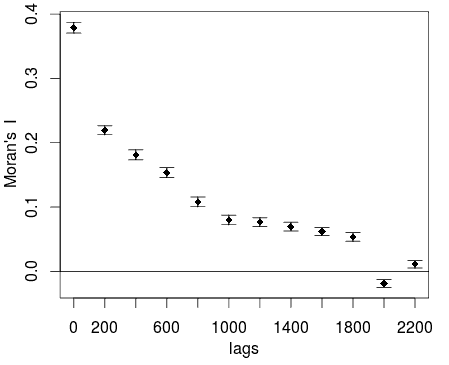
\includegraphics[width=0.45\textwidth]{pre_avg_NDVI_max_full}
\caption{Distance decay of NDVI values in 1999.}
  \label{DDFig}
\end{wrapfigure}

First, we use the Moran's I measurements (eq. \ref{EQmoran}) to select a buffer radius to use in the estimation of each individual project location.
As Figure \ref{DDFig} illustrates, the distance-decay function of NDVI in 1999 follows an expected pattern, with spatial autocorrelation dropping off as distances increase.  
We use this information to select a buffer radius of 800 kilometers as our threshold (Moran's I ~= .10).  
For each unit of analysis we then draw a subpopulation of all World Bank projects which fall within the 800km radius.

\par
For each of these 13769 subpopulations, we match control and treatment cases on the basis of the propensity scores estimated in eq.\ref{EQpropensity}, following a nearest-neighbor matching strategy.  
A caliper of .25 is used to exclude poor matches, and after matching if a sufficient total of matches does not exist (less than 30 total matches), the unit is excluded from analysis and we move to the next subpopulation. 
\par

\begin{wrapfigure}[23]{r}{0.75\textwidth}\centering
\begin{Schunk}

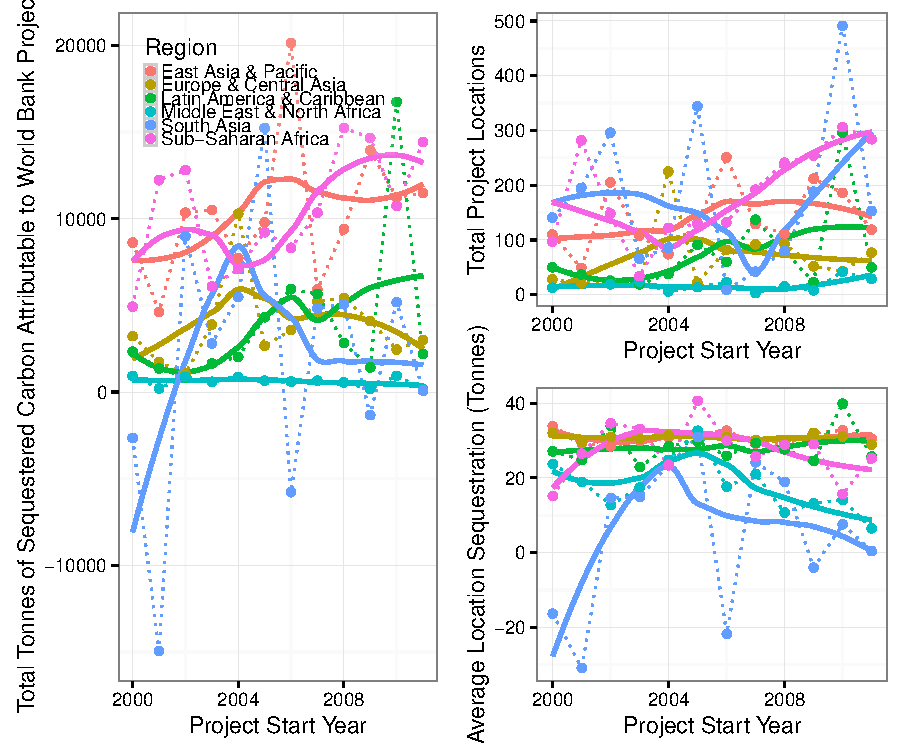
\includegraphics[width=\maxwidth]{figure/Fig1-1} \end{Schunk}
\caption{Results from estimates by region and time.}
\label{result_fig}
\vspace{10pt}
\end{wrapfigure}  

After matching is conducted for each subpopulation, a regression is performed for that subpopulation following eq.\ref{EQgwr}.  
This results in 8399 projects which have adequate matches for estimation, or 61\% of all large scale projects. 
For each of these models, we record all relevant information regarding standard errors and estimated coefficients, and provide an interface for users to examine these values across all models\footnote{A fully interactive online tool to explore results is available, but is omitted from this submission to facilitate blind peer review.}.  
The impacts estimated for each of these project locations (\begin{math}\theta\end{math} in eq. \ref{EQgwr}) are entered in to the fixed-effect model derived following eq. \ref{EQcarb} (a total of 60 fixed effects estimates are derived in this model, representing all ecofloristic zones which contained World Bank projects).
This provides a regionally-specific estimate of the tonnes of carbon sequestered attributable to a World Bank project.
A region- and temporal- disaggregation of the results across all estimated projects can be seen in Figure \ref{result_fig}.

\newpage
\section{Discussion}
The approach outlined in this document highlights a number of interesting findings, but is constrained by significant limitations on methodologic fronts.
Of the key findings, we highlight the general improvement of World Bank projects over time, most notably in south Asia - a trend which could be reflective of functional environmental safeguards.  
However, we also highlight the significant geographic variation in this finding.  For example, development projects in India almost universally had relatively negative impacts on sequestration, while those in the Philippines had relatively positive impacts.  
This is also evident on a region-by-region basis, as the negative trend line within the Middle East and North Africa highlights (see Figure \ref{result_fig}).  
\par
This approach has the benefit of contrasting World Bank project locations to other locations at which it is known a World Bank project (albeit of a small magnitude) exists, and comparisons are conducted within projects that are - at least - known to be within the same sector. 
Further, by leveraging the geographic context in which projects exist, this approach has the potential to improve matches by providing pairs which are contextually similar - i.e., projects in dense forests are compared to other projects in dense forests; those near urban areas and contrasted to others near urban areas.
Both of these attributes help to mitigate concerns over omitted variable biases, though come with drawbacks noted below.
Lastly, by leveraging the geographically-explicit approach detailed here, each project location receives an estimated impact.
While interaction terms can provide some insights into heterogeneous effects, the geographic limitations on subpopulations provide unique insights into trends that may vary over space.
\par
Many opportunities exist to advance research which seeks to incorporate geographic data into models which causally identify impacts.
First and foremost are the well known disadvantages to geographically weighted regression (GWR) approaches - namely spatial correlation in estimated coefficients, bias in standard error terms (\cite{wheeler_multicollinearity_2005}), and the necessity to define a weights matrix (i.e., in this piece we choose a Moran's I threshold of 0.1 to approximate a single threshold).  
These factors limit the interpretation of the estimates calculated in this paper, specifically preventing insights into the overall significant or treatment impact across multiple locations - i.e., individual estimates can be interpreted, but aggregate estimates which rely on statistical significance can be misleading.
Ongoing research is examining potential solutions to this problem - for example, leveraging the techniques of Seemingly Unrelated Regression (SURE) or the emergent causal machine learning approaches (see \cite{athey_recursive_2015}), but much of this research is currently nascent - and solutions appear to be extremely computationally intensive.
\par
A second limitation of this approach is in the matching strategy employed.
Because we chose to contrast high-dollar value World Bank projects to low-dollar value World Bank projects within the same sector, we have a higher degree of confidence in a reduced omission bias - i.e., it is more likely we're comparing "apples to apples".
However, this also significantly limited the number of adequate matches which could be found, leading to a lack of estimates for approximately 40\% of project locations.
This is representative of a broader concern of any top-down approaches to impact evaluation, as there is frequently limited information on the characteristics of the project and relevant geographic contextual factors to include.
Ongoing research into key characteristics of projects (i.e., beyond the number of dollars allocated and sectoral grouping) seeks to mitigate these concerns, and provide increasingly better matches when top-down strategies are pursued.
\par
Despite these limitations, we believe this approach provides policymakers with a cost-effective approach to rapidly assessing a very large portfolio of projects to identify "warning flags" or "bright spots".  
We do not suggest that such analyses take the place of traditional impact evaluation strategies, but rather argue that top-down analyses such as these can help better direct resources for more rigorous, in-situ assessments.
Further, because we leverage satellite information which is regularly updated, such strategies could be applied not only to project evaluation, but also project monitoring.
\par
Following this, we argue that sub-national data can be helpful in the identification of  heterogeneous impact effects. 
This piece highlights this by examining the impact of large scale World Bank projects on carbon sequestration at a global scale.  
We find that while projects have had an overall positive effect, significant temporal and geographic variation exists.
Finally, we argue for the importance of further research into methods to estimate geographically heterogeneous impacts effects.
\newpage

\section{Acknowledgements}
The authors would like to acknowledge the government of Sweden and the World Bank Independent Evaluation Group for partially funding this research.  
This work was performed in part using computational facilities at the College of William and Mary which were provided with the assistance of the National Science Foundation, Virginia Port Authority, Virginia's Commonwealth Technology Research Fund, and the Office of Naval Research.  
The authors would also like to thank Scott Stewart, Alex Kappel, Zhonghui Lv, Doug Nicholson, and Vinay Vijayan for their valuable contributions and insights.


\newpage
%Need to ensure formatting is correct -
%http://endnote.com/downloads/style/conservation-letters
%Limited to 40 references
\printbibliography



\end{knitrout}
\end{document}
